\chapter{Súčasný stav problematiky}

Tu je potrebné popísať doteraz získané poznatky z problematiky. 
Nezabudnúť dôsledne citovať autorov článkov, kníh aj internetových publikácií 
napr. monografia \cite{berman}. 
V prameňoch -- spravidla posledná kapitola -- treba uviesť všetku použitú literatúru. 
Nemala by obsahovať tie zdroje, ktoré nie sú v práci citované.
A tiež nie je vhodné citovať nedôveryhodné zdroje ako sú Wikipédia ap.

Na obrázku \ref{obr1} máme príklad zo zábavnej matematiky uvedený v práci Peško \cite{pes2}.

\begin{figure}[ht]
\begin{center}
\begin{minipage}{0.7\linewidth}
\begin{center}
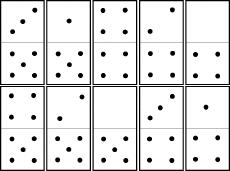
\includegraphics[width=.8\textwidth]{domino.jpg}
\caption{Ako popreklápať kocky domina tak, aby rozdiel medzi 
súčtami horných a dolných políčok bol čo najmenší? }
\label{obr1}
\end{center}
\end{minipage}
\end{center}
\end{figure}

Alebo dva obrázky vedľa seba:

\begin{figure}[ht]
\phantom.\hfill
%
\begin{minipage}{0.4\linewidth}
\begin{center}
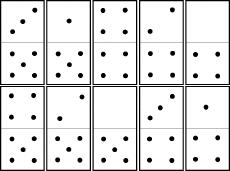
\includegraphics[width=.8\textwidth]{domino.jpg}
\caption{Názov ľavého obrázku}
\label{obrL1}
\end{center}
\end{minipage}
%
\hfill
%
\begin{minipage}{0.4\linewidth}
\begin{center}
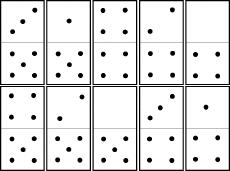
\includegraphics[width=.8\textwidth]{domino.jpg}
\caption{Názov pravého obrázku}
\label{obrP1}
\end{center}
\end{minipage}
%
\hfill\phantom.
\end{figure}



Matematicky možeme vzťahy označiť:

\begin{equation} 
\label{nerov1}
c_{i,j}^2+c_{k,l} \le \frac{c_{i,l}}{c_{k,j}}
\end{equation}

a potom sa naň neskôr v texte~\eqref{nerov1} odvolávať. Ak sa pri reporte objavia symboly 
(??) treba zopakovať \verb|pdflatex praca|.


Môžeme použiť aj iné matematické prostredia:

$$
c_{i,j}^2+c_{k,l} \le \frac{c_{i,l}}{c_{k,j}}
$$

resp.

\begin{displaymath}
c_{i,j}^2+c_{k,l} \le \frac{c_{i,l}}{c_{k,j}}
\end{displaymath}

resp.

\begin{equation*} 
c_{i,j}^2+c_{k,l} \le \frac{c_{i,l}}{c_{k,j}}
\end{equation*}

resp.

\begin{multline*}
c_{i,j}^2+c_{k,l} \le \frac{c_{i,l}}{c_{k,j}} \cdots \mbox{riadok číslo 1} \allowdisplaybreaks\\
c_{i,j}^2+c_{k,l} \le \frac{c_{i,l}}{c_{k,j}} \cdots \mbox{riadok číslo 2} \allowdisplaybreaks\\
c_{i,j}^2+c_{k,l} \le \frac{c_{i,l}}{c_{k,j}} \cdots \mbox{riadok číslo 3} \allowdisplaybreaks\\
c_{i,j}^2+c_{k,l} \le \frac{c_{i,l}}{c_{k,j}} \cdots \mbox{riadok číslo 4}
\end{multline*}

resp.

\begin{multline}
c_{i,j}^2+c_{k,l} \le \frac{c_{i,l}}{c_{k,j}} \cdots \mbox{riadok číslo 1} \\
c_{i,j}^2+c_{k,l} \le \frac{c_{i,l}}{c_{k,j}} \cdots \mbox{riadok číslo 2} \\
c_{i,j}^2+c_{k,l} \le \frac{c_{i,l}}{c_{k,j}} \cdots \mbox{riadok číslo 3} \\
c_{i,j}^2+c_{k,l} \le \frac{c_{i,l}}{c_{k,j}} \cdots \mbox{riadok číslo 4}
\label{vztah-22}
\end{multline}

resp.

\begin{eqnarray*}
c_{i,j}^2+c_{k,l} &\le& \frac{c_{i,l}}{c_{k,j}} \cdots \mbox{riadok číslo 1} \\
c_{i,j}^2+c_{k,l} &\le& \frac{c_{i,l}}{c_{k,j}} \cdots \mbox{riadok číslo 2} \\
c_{i,j}^2+c_{k,l} &\le& \frac{c_{i,l}}{c_{k,j}} \cdots \mbox{riadok číslo 3} \\
c_{i,j}^2+c_{k,l} \le  &xxx& \frac{c_{i,l}}{c_{k,j}} \cdots \mbox{riadok číslo 4}
\end{eqnarray*}

resp.

\begin{eqnarray}
\label{xx01}
c_{i,j}^2+c_{k,l} &\le& \frac{c_{i,l}}{c_{k,j}} \cdots \mbox{riadok číslo 1} \\
\label{xx02}
c_{i,j}^2+c_{k,l} &\le& \frac{c_{i,l}}{c_{k,j}} \cdots \mbox{riadok číslo 2} \\
\label{xx03}\nonumber
c_{i,j}^2+c_{k,l} &\le& \frac{c_{i,l}}{c_{k,j}} \cdots \mbox{riadok číslo 3} \\
\label{xx04}
c_{i,j}^2+c_{k,l} &xxx& \frac{c_{i,l}}{c_{k,j}} \cdots \mbox{riadok číslo 4}
\end{eqnarray}



\noindent
Niekedy sa hodí pracovať s maticami alebo determinantami:

$$
{\mathbb A} = 
\left( \begin{array}{@{}*{3}{r}@{}}
-5 &  8 &  3\\
 0 & -0 &  2\\
 5 &  1 & -2  
\end{array} \right)
%
\times
%
\left[ \begin{array}{@{}*{3}{c}@{}}
-5 &  8 &  3\\
 0 & -0 &  2\\
 5 &  1 & -2  
\end{array} \right\}
%
+
%
\left| \begin{array}{@{}*{3}{r}@{}}
-5 &  8 &  3\\
 0 & -0 &  2\\
 5 &  1 & -2  
\end{array} \right\vert
%
+
%
\left\Vert\begin{array}{@{}*{3}{c}@{}}
-5 & 8,1  & 3,4 \\
x  & -0,2 & 2   \\
5  & 1    & -2  
\end{array} \right\Vert
$$

\begin{figure}[ht]
\begin{center}
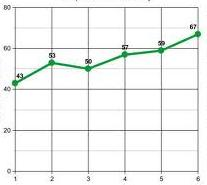
\includegraphics[width=.4\textwidth]{obrazok.jpg}
\caption{Obrázok}
\label{obr2}
\end{center}
\end{figure}

Tu je potrebné popísať doteraz získané poznatky z problematiky. 
Nezabudnúť dôsledne citovať autorov článkov, kníh aj internetových publikácií 
napr. monografia \cite{pes2, berman}. 

Na obrázku \ref{obr1a} máme príklad zo zábavnej matematiky uvedený v práci Peško \cite{pes2}.
Porovnajte definíciu, zobrazenie a tiež umiestnenie obrázku \ref{obr1a} s obrázkom \ref{obr1}.

\begin{figure}[ht]
\begin{center}
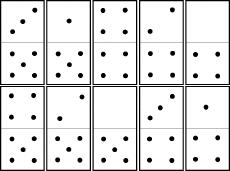
\includegraphics[width=.5\textwidth]{domino.jpg}
\caption{Ako popreklápať kocky domina tak, aby rozdiel medzi 
súčtami horných a dolných políčok bol čo najmenší? }
\label{obr1a}
\end{center}
\end{figure}

